\subsection{分布评分改善不保证均值位置更准}
300秒观测间隔程序体现了这一区别：相对具名Full01对照，加权ES变化为
$-23.40$米，FDE却变化为$+9.64$米。表\ref{tab:point-errors}中它在四个保存目标的
均值位置误差也都更大。ES同时涉及粒子到目标的距离和粒子之间的离散程度，
不能换算成均值位置误差。观测间隔比较还改变训练暴露与扩散绑定，
因而不隔离数值积分本身的作用。

\begin{figure}[htbp]\centering
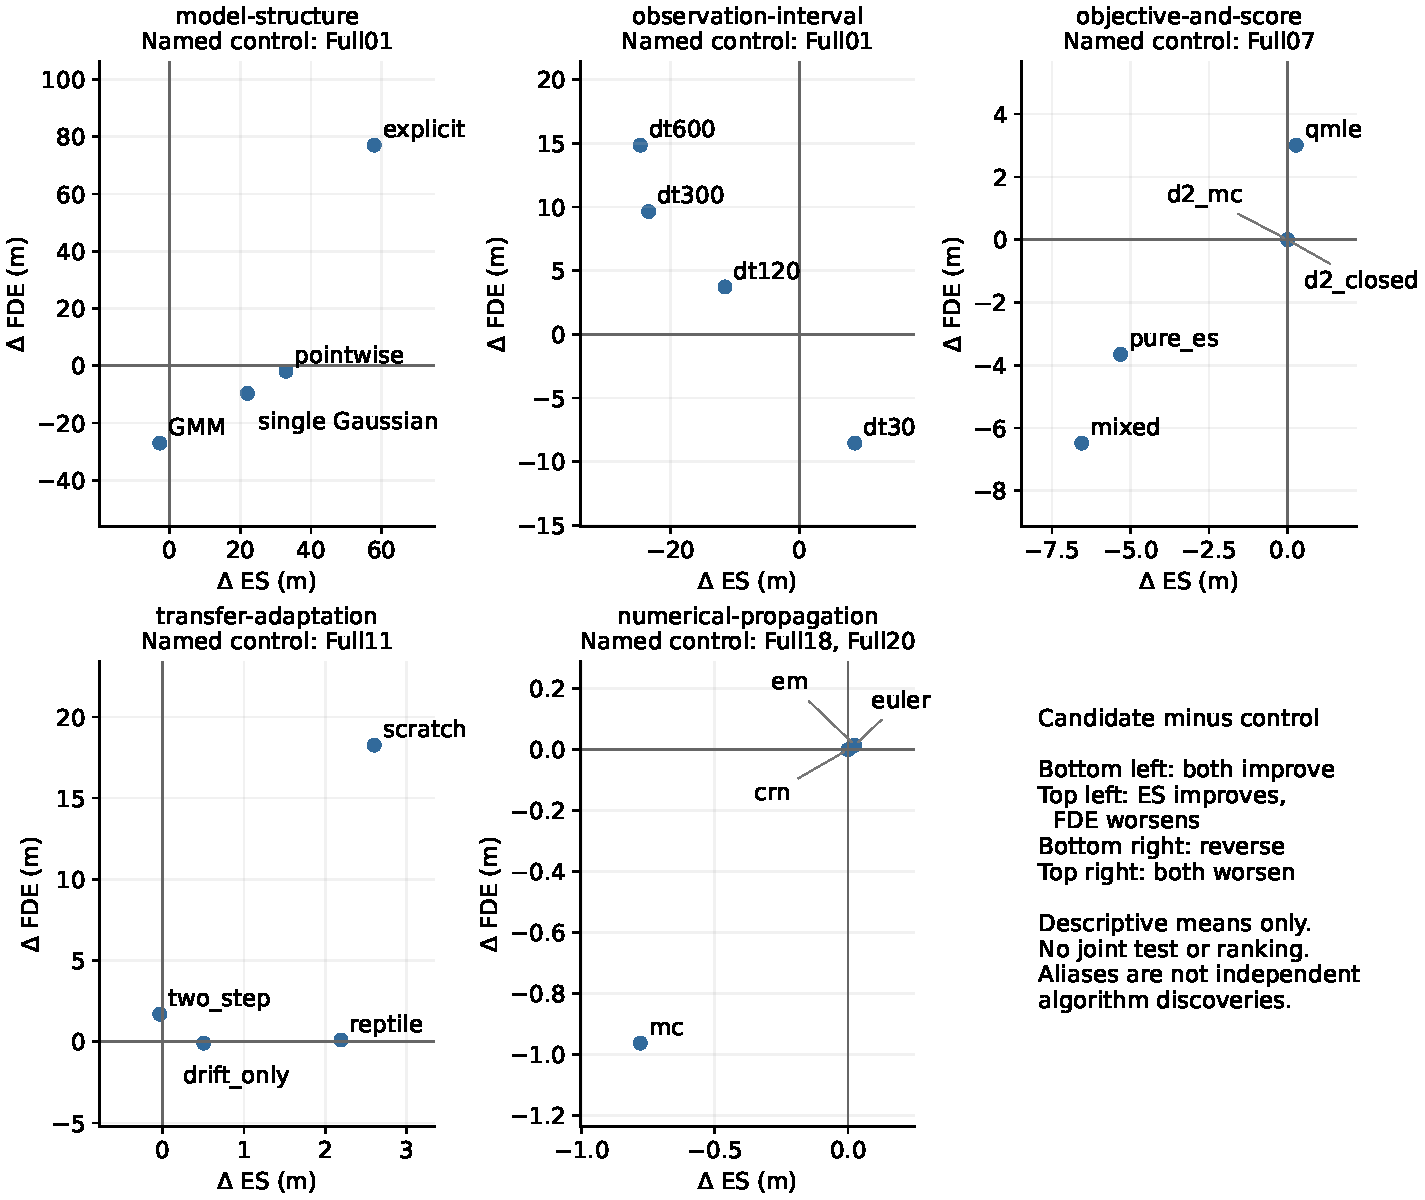
\includegraphics[width=\linewidth]{../figures/reader-v2/tradeoff.pdf}
\caption{分布评分与终点误差取舍。全部21比较编码42个差值标量，保留五登记家族与具名对照。
每点先在46个配对块各自平均五种子，再等权平均块；ES先平均四目标，FDE只取末目标。
两轴负差有利；左上象限表示ES改善而FDE变差。各分面尺度不同。
这些均值没有联合置信区域，不能建立Pareto优势或全局算法排名。}
\label{fig:reader-tradeoff}\end{figure}
dt300的ES同时区间为$[-48.27,-2.47]$米。虽不跨零，仍未满足登记实际有益条件：
整个区间须低于$-41.100259$米并通过其他门槛。
因此该点说明指标冲突，不说明已达到实际优越性；所有差值均用未舍入源值计算。
